\documentclass[]{article}
\usepackage{lmodern}
\usepackage{amssymb,amsmath}
\usepackage{ifxetex,ifluatex}
\usepackage{fixltx2e} % provides \textsubscript
\ifnum 0\ifxetex 1\fi\ifluatex 1\fi=0 % if pdftex
  \usepackage[T1]{fontenc}
  \usepackage[utf8]{inputenc}
\else % if luatex or xelatex
  \ifxetex
    \usepackage{mathspec}
  \else
    \usepackage{fontspec}
  \fi
  \defaultfontfeatures{Ligatures=TeX,Scale=MatchLowercase}
\fi
% use upquote if available, for straight quotes in verbatim environments
\IfFileExists{upquote.sty}{\usepackage{upquote}}{}
% use microtype if available
\IfFileExists{microtype.sty}{%
\usepackage{microtype}
\UseMicrotypeSet[protrusion]{basicmath} % disable protrusion for tt fonts
}{}
\usepackage[margin=1in]{geometry}
\usepackage{hyperref}
\hypersetup{unicode=true,
            pdftitle={Homework 04},
            pdfauthor={Weiling Li},
            pdfborder={0 0 0},
            breaklinks=true}
\urlstyle{same}  % don't use monospace font for urls
\usepackage{color}
\usepackage{fancyvrb}
\newcommand{\VerbBar}{|}
\newcommand{\VERB}{\Verb[commandchars=\\\{\}]}
\DefineVerbatimEnvironment{Highlighting}{Verbatim}{commandchars=\\\{\}}
% Add ',fontsize=\small' for more characters per line
\usepackage{framed}
\definecolor{shadecolor}{RGB}{248,248,248}
\newenvironment{Shaded}{\begin{snugshade}}{\end{snugshade}}
\newcommand{\AlertTok}[1]{\textcolor[rgb]{0.94,0.16,0.16}{#1}}
\newcommand{\AnnotationTok}[1]{\textcolor[rgb]{0.56,0.35,0.01}{\textbf{\textit{#1}}}}
\newcommand{\AttributeTok}[1]{\textcolor[rgb]{0.77,0.63,0.00}{#1}}
\newcommand{\BaseNTok}[1]{\textcolor[rgb]{0.00,0.00,0.81}{#1}}
\newcommand{\BuiltInTok}[1]{#1}
\newcommand{\CharTok}[1]{\textcolor[rgb]{0.31,0.60,0.02}{#1}}
\newcommand{\CommentTok}[1]{\textcolor[rgb]{0.56,0.35,0.01}{\textit{#1}}}
\newcommand{\CommentVarTok}[1]{\textcolor[rgb]{0.56,0.35,0.01}{\textbf{\textit{#1}}}}
\newcommand{\ConstantTok}[1]{\textcolor[rgb]{0.00,0.00,0.00}{#1}}
\newcommand{\ControlFlowTok}[1]{\textcolor[rgb]{0.13,0.29,0.53}{\textbf{#1}}}
\newcommand{\DataTypeTok}[1]{\textcolor[rgb]{0.13,0.29,0.53}{#1}}
\newcommand{\DecValTok}[1]{\textcolor[rgb]{0.00,0.00,0.81}{#1}}
\newcommand{\DocumentationTok}[1]{\textcolor[rgb]{0.56,0.35,0.01}{\textbf{\textit{#1}}}}
\newcommand{\ErrorTok}[1]{\textcolor[rgb]{0.64,0.00,0.00}{\textbf{#1}}}
\newcommand{\ExtensionTok}[1]{#1}
\newcommand{\FloatTok}[1]{\textcolor[rgb]{0.00,0.00,0.81}{#1}}
\newcommand{\FunctionTok}[1]{\textcolor[rgb]{0.00,0.00,0.00}{#1}}
\newcommand{\ImportTok}[1]{#1}
\newcommand{\InformationTok}[1]{\textcolor[rgb]{0.56,0.35,0.01}{\textbf{\textit{#1}}}}
\newcommand{\KeywordTok}[1]{\textcolor[rgb]{0.13,0.29,0.53}{\textbf{#1}}}
\newcommand{\NormalTok}[1]{#1}
\newcommand{\OperatorTok}[1]{\textcolor[rgb]{0.81,0.36,0.00}{\textbf{#1}}}
\newcommand{\OtherTok}[1]{\textcolor[rgb]{0.56,0.35,0.01}{#1}}
\newcommand{\PreprocessorTok}[1]{\textcolor[rgb]{0.56,0.35,0.01}{\textit{#1}}}
\newcommand{\RegionMarkerTok}[1]{#1}
\newcommand{\SpecialCharTok}[1]{\textcolor[rgb]{0.00,0.00,0.00}{#1}}
\newcommand{\SpecialStringTok}[1]{\textcolor[rgb]{0.31,0.60,0.02}{#1}}
\newcommand{\StringTok}[1]{\textcolor[rgb]{0.31,0.60,0.02}{#1}}
\newcommand{\VariableTok}[1]{\textcolor[rgb]{0.00,0.00,0.00}{#1}}
\newcommand{\VerbatimStringTok}[1]{\textcolor[rgb]{0.31,0.60,0.02}{#1}}
\newcommand{\WarningTok}[1]{\textcolor[rgb]{0.56,0.35,0.01}{\textbf{\textit{#1}}}}
\usepackage{graphicx,grffile}
\makeatletter
\def\maxwidth{\ifdim\Gin@nat@width>\linewidth\linewidth\else\Gin@nat@width\fi}
\def\maxheight{\ifdim\Gin@nat@height>\textheight\textheight\else\Gin@nat@height\fi}
\makeatother
% Scale images if necessary, so that they will not overflow the page
% margins by default, and it is still possible to overwrite the defaults
% using explicit options in \includegraphics[width, height, ...]{}
\setkeys{Gin}{width=\maxwidth,height=\maxheight,keepaspectratio}
\IfFileExists{parskip.sty}{%
\usepackage{parskip}
}{% else
\setlength{\parindent}{0pt}
\setlength{\parskip}{6pt plus 2pt minus 1pt}
}
\setlength{\emergencystretch}{3em}  % prevent overfull lines
\providecommand{\tightlist}{%
  \setlength{\itemsep}{0pt}\setlength{\parskip}{0pt}}
\setcounter{secnumdepth}{0}
% Redefines (sub)paragraphs to behave more like sections
\ifx\paragraph\undefined\else
\let\oldparagraph\paragraph
\renewcommand{\paragraph}[1]{\oldparagraph{#1}\mbox{}}
\fi
\ifx\subparagraph\undefined\else
\let\oldsubparagraph\subparagraph
\renewcommand{\subparagraph}[1]{\oldsubparagraph{#1}\mbox{}}
\fi

%%% Use protect on footnotes to avoid problems with footnotes in titles
\let\rmarkdownfootnote\footnote%
\def\footnote{\protect\rmarkdownfootnote}

%%% Change title format to be more compact
\usepackage{titling}

% Create subtitle command for use in maketitle
\providecommand{\subtitle}[1]{
  \posttitle{
    \begin{center}\large#1\end{center}
    }
}

\setlength{\droptitle}{-2em}

  \title{Homework 04}
    \pretitle{\vspace{\droptitle}\centering\huge}
  \posttitle{\par}
  \subtitle{Generalized Linear Models}
  \author{Weiling Li}
    \preauthor{\centering\large\emph}
  \postauthor{\par}
      \predate{\centering\large\emph}
  \postdate{\par}
    \date{October 14, 2019}


\begin{document}
\maketitle

\begin{Shaded}
\begin{Highlighting}[]
\NormalTok{knitr}\OperatorTok{::}\NormalTok{opts_chunk}\OperatorTok{$}\KeywordTok{set}\NormalTok{(}\DataTypeTok{echo =} \OtherTok{TRUE}\NormalTok{,}\DataTypeTok{out.width=}\StringTok{"0.9}\CharTok{\textbackslash{}\textbackslash{}}\StringTok{linewidth"}\NormalTok{,}\DataTypeTok{dev=}\StringTok{"pdf"}\NormalTok{,}\DataTypeTok{fig.align  =} \StringTok{'center'}\NormalTok{)}
\NormalTok{knitr}\OperatorTok{::}\NormalTok{opts_chunk}\OperatorTok{$}\KeywordTok{set}\NormalTok{(}\DataTypeTok{warning =} \OtherTok{FALSE}\NormalTok{)}
\NormalTok{pacman}\OperatorTok{::}\KeywordTok{p_load}\NormalTok{(}\StringTok{"knitr"}\NormalTok{,}\StringTok{"faraway"}\NormalTok{,}\StringTok{"arm"}\NormalTok{,}\StringTok{"hett"}\NormalTok{,}\StringTok{"data.table"}\NormalTok{,}\StringTok{"foreign"}\NormalTok{,}\StringTok{"car"}\NormalTok{,}\StringTok{"VGAM"}\NormalTok{,}\StringTok{"MASS"}\NormalTok{,}\StringTok{"censReg"}\NormalTok{,}\StringTok{"tidyverse"}\NormalTok{)}
\end{Highlighting}
\end{Shaded}

\hypertarget{data-analysis}{%
\section{Data analysis}\label{data-analysis}}

\hypertarget{poisson-regression}{%
\subsection{Poisson regression:}\label{poisson-regression}}

The folder \emph{risky.behavior} contains data from a randomized trial
targeting couples at high risk of HIV infection. The intervention
provided counseling sessions regarding practices that could reduce their
likelihood of contracting HIV. Couples were randomized either to a
control group, a group in which just the woman participated, or a group
in which both members of the couple participated. One of the outcomes
examined after three months was ``number of unprotected sex acts''.

\begin{Shaded}
\begin{Highlighting}[]
\NormalTok{risky_behaviors<-}\KeywordTok{read.dta}\NormalTok{(}\StringTok{"http://www.stat.columbia.edu/~gelman/arm/examples/risky.behavior/risky_behaviors.dta"}\NormalTok{)}
\end{Highlighting}
\end{Shaded}

\begin{enumerate}
\def\labelenumi{\arabic{enumi}.}
\tightlist
\item
  Model this outcome as a function of treatment assignment using a
  Poisson regression. Does the model fit well? Is there evidence of
  overdispersion?
\end{enumerate}

\begin{Shaded}
\begin{Highlighting}[]
\KeywordTok{ggplot}\NormalTok{(risky_behaviors)}\OperatorTok{+}\KeywordTok{aes}\NormalTok{(fupacts)}\OperatorTok{+}\KeywordTok{geom_histogram}\NormalTok{(}\DataTypeTok{bins =} \DecValTok{30}\NormalTok{)}
\end{Highlighting}
\end{Shaded}

\begin{center}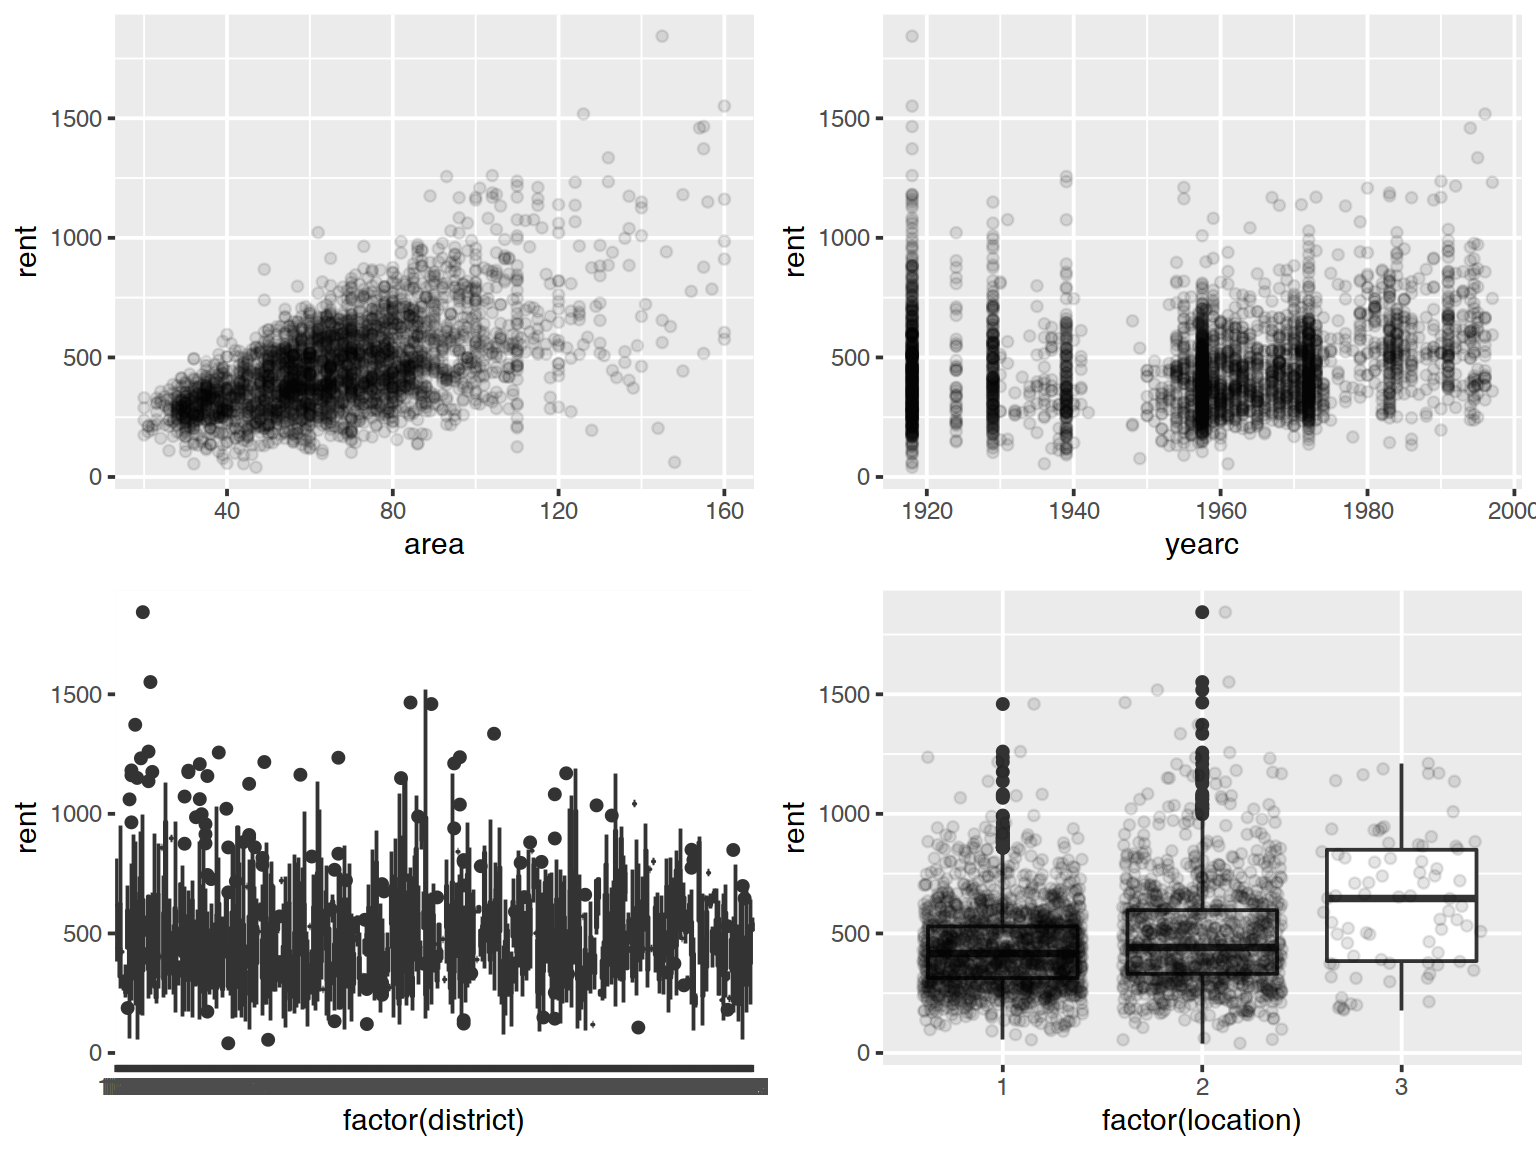
\includegraphics[width=0.9\linewidth]{hw_glm_2018_files/figure-latex/unnamed-chunk-2-1} \end{center}

\begin{Shaded}
\begin{Highlighting}[]
\NormalTok{fit}\FloatTok{.1}\NormalTok{ =}\StringTok{ }\KeywordTok{glm}\NormalTok{(}\DataTypeTok{data =}\NormalTok{ risky_behaviors,fupacts }\OperatorTok{~}\StringTok{ }\NormalTok{couples}\OperatorTok{+}\NormalTok{women_alone,}\DataTypeTok{family =} \KeywordTok{poisson}\NormalTok{(}\DataTypeTok{link =} \StringTok{"log"}\NormalTok{))}
\KeywordTok{ggplot}\NormalTok{(fit}\FloatTok{.1}\NormalTok{)}\OperatorTok{+}\KeywordTok{aes}\NormalTok{(}\DataTypeTok{x =}\NormalTok{ .fitted,}\DataTypeTok{y =}\NormalTok{ .stdresid)}\OperatorTok{+}\KeywordTok{geom_point}\NormalTok{()}\OperatorTok{+}\KeywordTok{geom_abline}\NormalTok{(}\DataTypeTok{intercept =} \FloatTok{2.0}\NormalTok{,}\DataTypeTok{slope =} \FloatTok{0.0}\NormalTok{)}\OperatorTok{+}\KeywordTok{geom_abline}\NormalTok{(}\DataTypeTok{intercept =} \FloatTok{-2.0}\NormalTok{,}\DataTypeTok{slope =} \FloatTok{0.0}\NormalTok{)}
\end{Highlighting}
\end{Shaded}

\begin{center}\includegraphics[width=0.9\linewidth]{hw_glm_2018_files/figure-latex/unnamed-chunk-2-2} \end{center}

\begin{Shaded}
\begin{Highlighting}[]
\KeywordTok{summary}\NormalTok{(fit}\FloatTok{.1}\NormalTok{)}
\end{Highlighting}
\end{Shaded}

\begin{verbatim}
## 
## Call:
## glm(formula = fupacts ~ couples + women_alone, family = poisson(link = "log"), 
##     data = risky_behaviors)
## 
## Deviance Residuals: 
##     Min       1Q   Median       3Q      Max  
## -6.6306  -4.9761  -3.2026   0.9829  27.1593  
## 
## Coefficients:
##             Estimate Std. Error z value Pr(>|z|)    
## (Intercept)  3.09024    0.01900  162.63   <2e-16 ***
## couples     -0.32263    0.02736  -11.79   <2e-16 ***
## women_alone -0.57409    0.03024  -18.99   <2e-16 ***
## ---
## Signif. codes:  0 '***' 0.001 '**' 0.01 '*' 0.05 '.' 0.1 ' ' 1
## 
## (Dispersion parameter for poisson family taken to be 1)
## 
##     Null deviance: 13307  on 433  degrees of freedom
## Residual deviance: 12931  on 431  degrees of freedom
## AIC: Inf
## 
## Number of Fisher Scoring iterations: 6
\end{verbatim}

Not really a good fit, there is a severe overdispersion in the model

\begin{enumerate}
\def\labelenumi{\arabic{enumi}.}
\setcounter{enumi}{1}
\tightlist
\item
  Next extend the model to include pre-treatment measures of the outcome
  and the additional pre-treatment variables included in the dataset.
  Does the model fit well? Is there evidence of overdispersion?
\end{enumerate}

\begin{Shaded}
\begin{Highlighting}[]
\NormalTok{fit}\FloatTok{.2}\NormalTok{ =}\StringTok{ }\KeywordTok{glm}\NormalTok{(}\DataTypeTok{data =}\NormalTok{ risky_behaviors,fupacts }\OperatorTok{~}\StringTok{ }\NormalTok{couples}\OperatorTok{+}\NormalTok{women_alone}\OperatorTok{+}\NormalTok{bs_hiv,}\DataTypeTok{family =} \KeywordTok{poisson}\NormalTok{(}\DataTypeTok{link =} \StringTok{"log"}\NormalTok{),}\DataTypeTok{offset =} \KeywordTok{log}\NormalTok{(bupacts}\OperatorTok{+}\DecValTok{1}\NormalTok{))}
\KeywordTok{ggplot}\NormalTok{(fit}\FloatTok{.2}\NormalTok{)}\OperatorTok{+}\KeywordTok{aes}\NormalTok{(}\DataTypeTok{x =}\NormalTok{ .fitted,}\DataTypeTok{y =}\NormalTok{ .stdresid)}\OperatorTok{+}\KeywordTok{geom_point}\NormalTok{()}\OperatorTok{+}\KeywordTok{geom_abline}\NormalTok{(}\DataTypeTok{intercept =} \FloatTok{2.0}\NormalTok{,}\DataTypeTok{slope =} \FloatTok{0.0}\NormalTok{)}\OperatorTok{+}\KeywordTok{geom_abline}\NormalTok{(}\DataTypeTok{intercept =} \FloatTok{-2.0}\NormalTok{,}\DataTypeTok{slope =} \FloatTok{0.0}\NormalTok{)}
\end{Highlighting}
\end{Shaded}

\begin{center}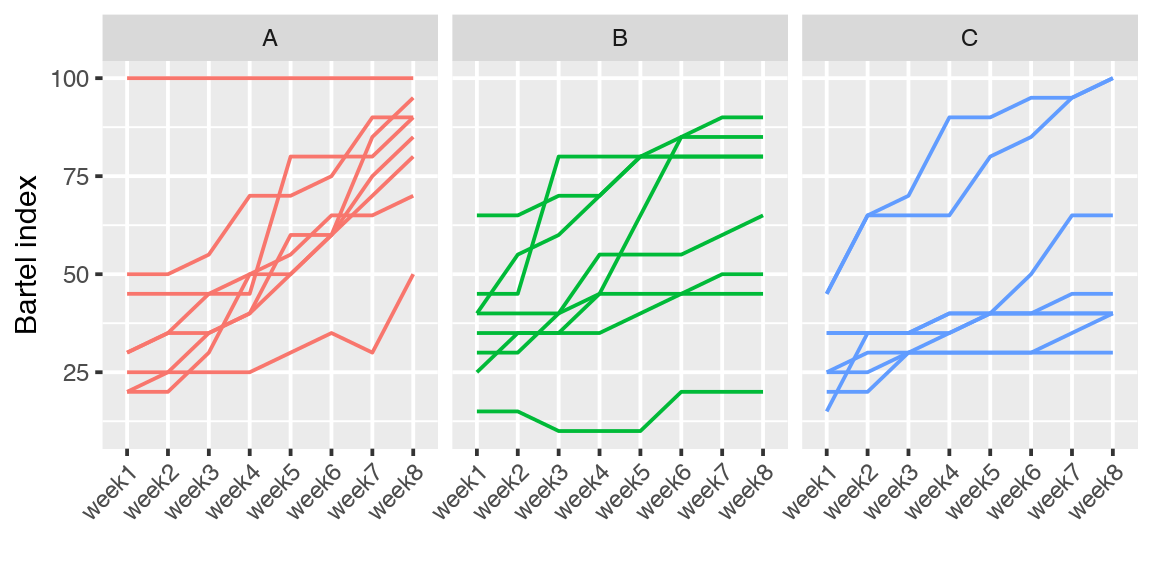
\includegraphics[width=0.9\linewidth]{hw_glm_2018_files/figure-latex/unnamed-chunk-3-1} \end{center}

\begin{Shaded}
\begin{Highlighting}[]
\KeywordTok{summary}\NormalTok{(fit}\FloatTok{.2}\NormalTok{)}
\end{Highlighting}
\end{Shaded}

\begin{verbatim}
## 
## Call:
## glm(formula = fupacts ~ couples + women_alone + bs_hiv, family = poisson(link = "log"), 
##     data = risky_behaviors, offset = log(bupacts + 1))
## 
## Deviance Residuals: 
##     Min       1Q   Median       3Q      Max  
## -16.573   -3.095   -1.224    1.807   21.062  
## 
## Coefficients:
##                Estimate Std. Error z value Pr(>|z|)    
## (Intercept)    -0.12615    0.01912  -6.599 4.14e-11 ***
## couples        -0.40297    0.02799 -14.396  < 2e-16 ***
## women_alone    -0.55145    0.03031 -18.192  < 2e-16 ***
## bs_hivpositive -0.31850    0.03547  -8.980  < 2e-16 ***
## ---
## Signif. codes:  0 '***' 0.001 '**' 0.01 '*' 0.05 '.' 0.1 ' ' 1
## 
## (Dispersion parameter for poisson family taken to be 1)
## 
##     Null deviance: 10433.9  on 433  degrees of freedom
## Residual deviance:  9914.1  on 430  degrees of freedom
## AIC: Inf
## 
## Number of Fisher Scoring iterations: 6
\end{verbatim}

from the residual plot, we can see that the model fit is better, but
over dispersion is still a severe problem for the fitted model.

\begin{enumerate}
\def\labelenumi{\arabic{enumi}.}
\setcounter{enumi}{2}
\tightlist
\item
  Fit an overdispersed Poisson model. What do you conclude regarding
  effectiveness of the intervention?
\end{enumerate}

\begin{Shaded}
\begin{Highlighting}[]
\NormalTok{fit}\FloatTok{.3}\NormalTok{ =}\StringTok{ }\KeywordTok{glm}\NormalTok{(}\DataTypeTok{data =}\NormalTok{ risky_behaviors,fupacts }\OperatorTok{~}\StringTok{ }\NormalTok{couples}\OperatorTok{+}\NormalTok{women_alone}\OperatorTok{+}\NormalTok{bs_hiv,}\DataTypeTok{family =} \KeywordTok{quasipoisson}\NormalTok{(}\DataTypeTok{link =} \StringTok{"log"}\NormalTok{),}\DataTypeTok{offset =} \KeywordTok{log}\NormalTok{(bupacts}\OperatorTok{+}\DecValTok{1}\NormalTok{))}
\KeywordTok{ggplot}\NormalTok{(fit}\FloatTok{.3}\NormalTok{)}\OperatorTok{+}\KeywordTok{aes}\NormalTok{(}\DataTypeTok{x =}\NormalTok{ .fitted,}\DataTypeTok{y =}\NormalTok{ .stdresid)}\OperatorTok{+}\KeywordTok{geom_point}\NormalTok{()}\OperatorTok{+}\KeywordTok{geom_abline}\NormalTok{(}\DataTypeTok{intercept =} \FloatTok{2.0}\NormalTok{,}\DataTypeTok{slope =} \FloatTok{0.0}\NormalTok{)}\OperatorTok{+}\KeywordTok{geom_abline}\NormalTok{(}\DataTypeTok{intercept =} \FloatTok{-2.0}\NormalTok{,}\DataTypeTok{slope =} \FloatTok{0.0}\NormalTok{)}
\end{Highlighting}
\end{Shaded}

\begin{center}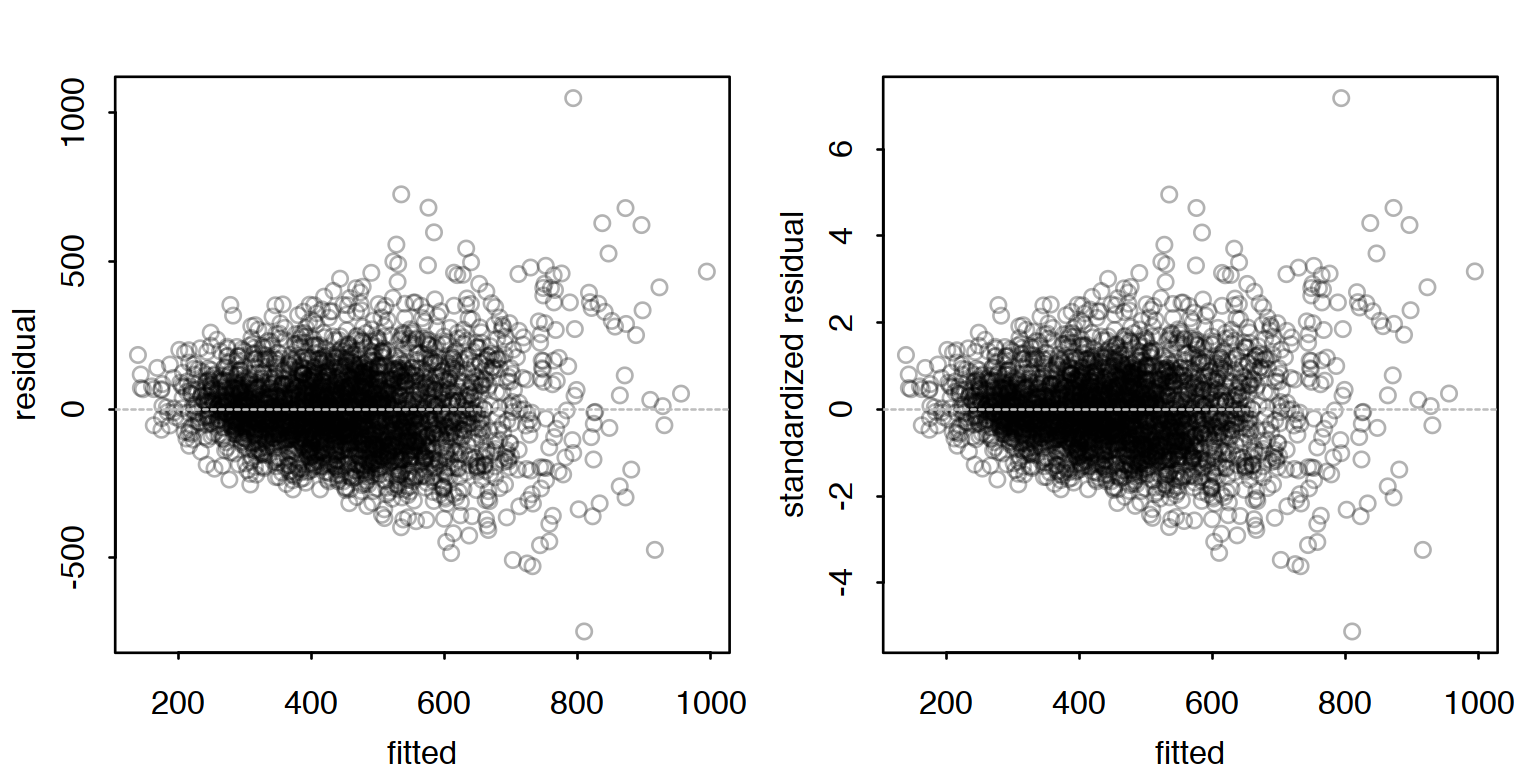
\includegraphics[width=0.9\linewidth]{hw_glm_2018_files/figure-latex/unnamed-chunk-4-1} \end{center}

\begin{Shaded}
\begin{Highlighting}[]
\KeywordTok{summary}\NormalTok{(fit}\FloatTok{.3}\NormalTok{)}
\end{Highlighting}
\end{Shaded}

\begin{verbatim}
## 
## Call:
## glm(formula = fupacts ~ couples + women_alone + bs_hiv, family = quasipoisson(link = "log"), 
##     data = risky_behaviors, offset = log(bupacts + 1))
## 
## Deviance Residuals: 
##     Min       1Q   Median       3Q      Max  
## -16.573   -3.095   -1.224    1.807   21.062  
## 
## Coefficients:
##                Estimate Std. Error t value Pr(>|t|)   
## (Intercept)     -0.1262     0.1213  -1.040  0.29900   
## couples         -0.4030     0.1776  -2.268  0.02379 * 
## women_alone     -0.5515     0.1924  -2.867  0.00435 **
## bs_hivpositive  -0.3185     0.2251  -1.415  0.15778   
## ---
## Signif. codes:  0 '***' 0.001 '**' 0.01 '*' 0.05 '.' 0.1 ' ' 1
## 
## (Dispersion parameter for quasipoisson family taken to be 40.27335)
## 
##     Null deviance: 10433.9  on 433  degrees of freedom
## Residual deviance:  9914.1  on 430  degrees of freedom
## AIC: NA
## 
## Number of Fisher Scoring iterations: 6
\end{verbatim}

from the model fit, the overall effectiveness of the intervention is
significant, with very dramatic change in rate of unprotected sex:
\(e^{-0.40 = 0.67}\) for couples and \(e^{-0.55} = 0.58\) for women only
and the statistical significance of the intervention is also sound.

\begin{enumerate}
\def\labelenumi{\arabic{enumi}.}
\setcounter{enumi}{3}
\tightlist
\item
  These data include responses from both men and women from the
  participating couples. Does this give you any concern withregard to
  our modeling assumptions?
\end{enumerate}

\begin{Shaded}
\begin{Highlighting}[]
\NormalTok{fit}\FloatTok{.4}\NormalTok{ =}\StringTok{ }\KeywordTok{glm}\NormalTok{(}\DataTypeTok{data =}\NormalTok{ risky_behaviors,fupacts }\OperatorTok{~}\StringTok{ }\NormalTok{sex}\OperatorTok{+}\NormalTok{couples}\OperatorTok{+}\NormalTok{women_alone}\OperatorTok{+}\NormalTok{bs_hiv,}\DataTypeTok{family =} \KeywordTok{quasipoisson}\NormalTok{(}\DataTypeTok{link =} \StringTok{"log"}\NormalTok{),}\DataTypeTok{offset =} \KeywordTok{log}\NormalTok{(bupacts}\OperatorTok{+}\DecValTok{1}\NormalTok{))}
\KeywordTok{ggplot}\NormalTok{(fit}\FloatTok{.4}\NormalTok{)}\OperatorTok{+}\KeywordTok{aes}\NormalTok{(}\DataTypeTok{x =}\NormalTok{ .fitted,}\DataTypeTok{y =}\NormalTok{ .stdresid)}\OperatorTok{+}\KeywordTok{geom_point}\NormalTok{()}\OperatorTok{+}\KeywordTok{geom_abline}\NormalTok{(}\DataTypeTok{intercept =} \FloatTok{2.0}\NormalTok{,}\DataTypeTok{slope =} \FloatTok{0.0}\NormalTok{)}\OperatorTok{+}\KeywordTok{geom_abline}\NormalTok{(}\DataTypeTok{intercept =} \FloatTok{-2.0}\NormalTok{,}\DataTypeTok{slope =} \FloatTok{0.0}\NormalTok{)}
\end{Highlighting}
\end{Shaded}

\begin{center}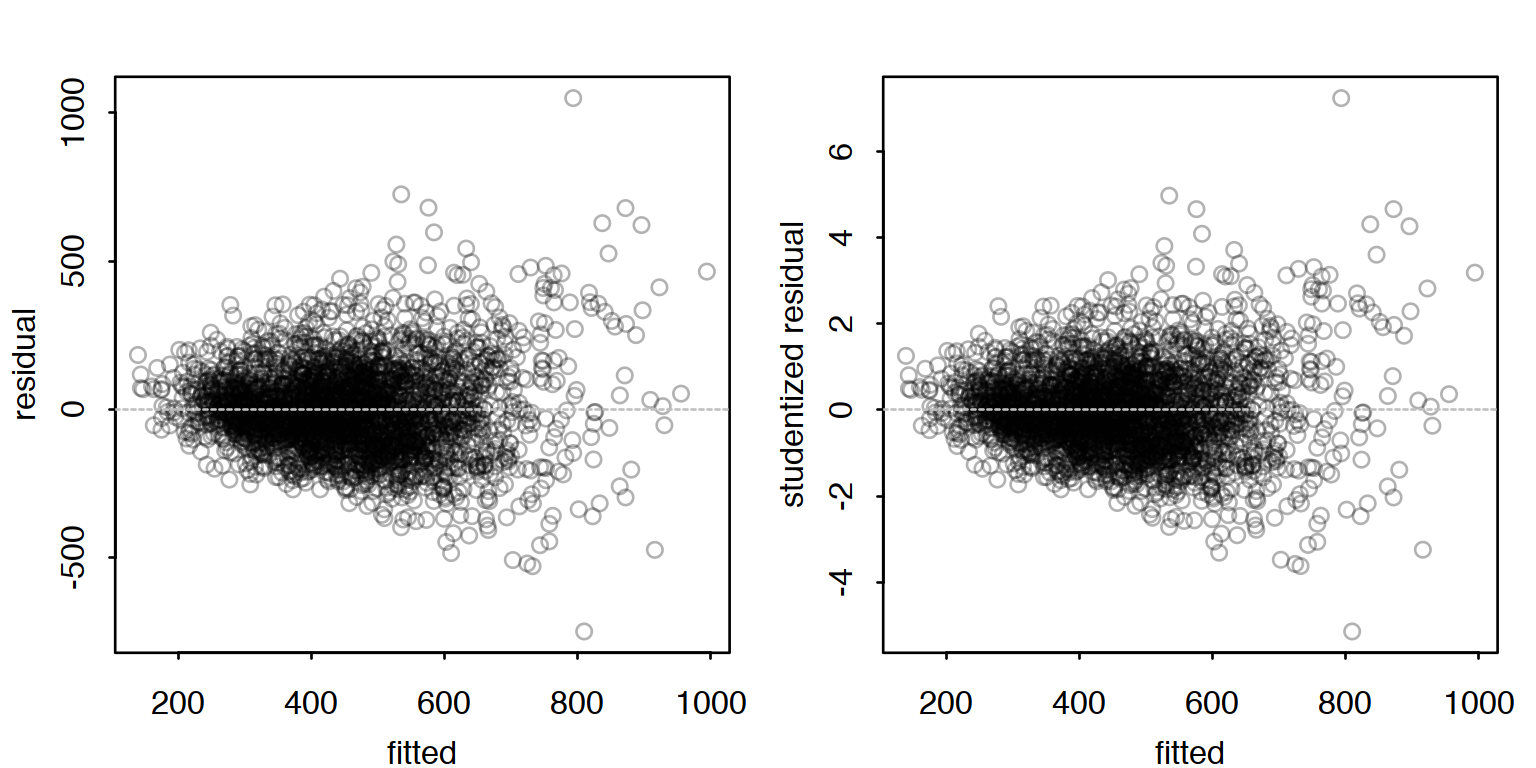
\includegraphics[width=0.9\linewidth]{hw_glm_2018_files/figure-latex/unnamed-chunk-5-1} \end{center}

\begin{Shaded}
\begin{Highlighting}[]
\KeywordTok{summary}\NormalTok{(fit}\FloatTok{.4}\NormalTok{)}
\end{Highlighting}
\end{Shaded}

\begin{verbatim}
## 
## Call:
## glm(formula = fupacts ~ sex + couples + women_alone + bs_hiv, 
##     family = quasipoisson(link = "log"), data = risky_behaviors, 
##     offset = log(bupacts + 1))
## 
## Deviance Residuals: 
##     Min       1Q   Median       3Q      Max  
## -16.040   -3.059   -1.171    1.785   21.494  
## 
## Coefficients:
##                Estimate Std. Error t value Pr(>|t|)   
## (Intercept)    -0.06692    0.14338  -0.467  0.64092   
## sexman         -0.11584    0.15112  -0.767  0.44377   
## couples        -0.40424    0.17866  -2.263  0.02416 * 
## women_alone    -0.55348    0.19360  -2.859  0.00446 **
## bs_hivpositive -0.32161    0.22641  -1.420  0.15621   
## ---
## Signif. codes:  0 '***' 0.001 '**' 0.01 '*' 0.05 '.' 0.1 ' ' 1
## 
## (Dispersion parameter for quasipoisson family taken to be 40.79777)
## 
##     Null deviance: 10433.9  on 433  degrees of freedom
## Residual deviance:  9890.1  on 429  degrees of freedom
## AIC: NA
## 
## Number of Fisher Scoring iterations: 6
\end{verbatim}

After testing the model with and without reporting sex, we found that
for this particular sample, male is associated with
\[1 - e^{-0.115} = 11%\] less unprotected sex reported but the
confidence of this claim is very weak.

One thing worth noted is that the residual showed some structure inside,
which means the model had fail to capture some structure of the data.

\hypertarget{comparing-logit-and-probit}{%
\section{Comparing logit and probit:}\label{comparing-logit-and-probit}}

Take one of the data examples from Chapter 5. Fit these data using both
logit and probit model. Check that the results are essentially the same
(after scaling by factor of 1.6)

\begin{Shaded}
\begin{Highlighting}[]
\NormalTok{brdata <-}\StringTok{ }\KeywordTok{read.dta}\NormalTok{(}\StringTok{"http://www.stat.columbia.edu/~gelman/arm/examples/nes/nes5200_processed_voters_realideo.dta"}\NormalTok{, }\DataTypeTok{convert.factors=}\NormalTok{F)}
\NormalTok{brdata <-}\StringTok{ }\NormalTok{brdata[}\KeywordTok{is.na}\NormalTok{(brdata}\OperatorTok{$}\NormalTok{black)}\OperatorTok{==}\OtherTok{FALSE}\OperatorTok{&}\KeywordTok{is.na}\NormalTok{(brdata}\OperatorTok{$}\NormalTok{female)}\OperatorTok{==}\OtherTok{FALSE}\OperatorTok{&}\KeywordTok{is.na}\NormalTok{(brdata}\OperatorTok{$}\NormalTok{educ1)}\OperatorTok{==}\OtherTok{FALSE}
\OperatorTok{&}\KeywordTok{is.na}\NormalTok{(brdata}\OperatorTok{$}\NormalTok{age)}\OperatorTok{==}\OtherTok{FALSE}\OperatorTok{&}\KeywordTok{is.na}\NormalTok{(brdata}\OperatorTok{$}\NormalTok{income)}\OperatorTok{==}\OtherTok{FALSE}\OperatorTok{&}\KeywordTok{is.na}\NormalTok{(brdata}\OperatorTok{$}\NormalTok{state)}\OperatorTok{==}\OtherTok{FALSE}\NormalTok{,]}
\NormalTok{kept.cases <-}\StringTok{ }\DecValTok{1952}\OperatorTok{:}\DecValTok{2000}
\NormalTok{matched.cases <-}\StringTok{ }\KeywordTok{match}\NormalTok{(brdata}\OperatorTok{$}\NormalTok{year, kept.cases)}
\NormalTok{keep <-}\StringTok{ }\OperatorTok{!}\KeywordTok{is.na}\NormalTok{(matched.cases)}
\NormalTok{data <-}\StringTok{ }\NormalTok{brdata[keep,]}
\NormalTok{income.new <-data}\OperatorTok{$}\NormalTok{income}\DecValTok{-3}


\NormalTok{rvote <-}\StringTok{ }\KeywordTok{ifelse}\NormalTok{ (data[,}\StringTok{"presvote"}\NormalTok{]}\OperatorTok{==}\DecValTok{1}\NormalTok{, }\DecValTok{0}\NormalTok{, }\KeywordTok{ifelse}\NormalTok{(data[,}\StringTok{"presvote"}\NormalTok{]}\OperatorTok{==}\DecValTok{2}\NormalTok{, }\DecValTok{1}\NormalTok{, }\OtherTok{NA}\NormalTok{))}

\NormalTok{fit}\FloatTok{.5}\NormalTok{ =}\StringTok{ }\KeywordTok{glm}\NormalTok{(rvote }\OperatorTok{~}\StringTok{ }\NormalTok{income.new,}\DataTypeTok{family =} \KeywordTok{binomial}\NormalTok{(}\DataTypeTok{link =} \StringTok{"logit"}\NormalTok{))}

\KeywordTok{curve}\NormalTok{ (}\KeywordTok{invlogit}\NormalTok{(fit}\FloatTok{.5}\OperatorTok{$}\NormalTok{coef[}\DecValTok{1}\NormalTok{] }\OperatorTok{+}\StringTok{ }\NormalTok{fit}\FloatTok{.5}\OperatorTok{$}\NormalTok{coef[}\DecValTok{2}\NormalTok{]}\OperatorTok{*}\NormalTok{x), }\DecValTok{-2}\NormalTok{, }\DecValTok{2}\NormalTok{, }\DataTypeTok{ylim=}\KeywordTok{c}\NormalTok{(}\OperatorTok{-}\NormalTok{.}\DecValTok{01}\NormalTok{,}\FloatTok{1.01}\NormalTok{),}
        \DataTypeTok{xlim=}\KeywordTok{c}\NormalTok{(}\OperatorTok{-}\DecValTok{4}\NormalTok{,}\DecValTok{4}\NormalTok{), }\DataTypeTok{xaxt=}\StringTok{"n"}\NormalTok{, }\DataTypeTok{xaxs=}\StringTok{"i"}\NormalTok{, }\DataTypeTok{mgp=}\KeywordTok{c}\NormalTok{(}\DecValTok{2}\NormalTok{,.}\DecValTok{5}\NormalTok{,}\DecValTok{0}\NormalTok{),}
        \DataTypeTok{ylab=}\StringTok{"Pr (Republican vote)"}\NormalTok{, }\DataTypeTok{xlab=}\StringTok{"Income"}\NormalTok{, }\DataTypeTok{lwd=}\DecValTok{4}\NormalTok{)}
\KeywordTok{curve}\NormalTok{ (}\KeywordTok{invlogit}\NormalTok{(fit}\FloatTok{.5}\OperatorTok{$}\NormalTok{coef[}\DecValTok{1}\NormalTok{] }\OperatorTok{+}\StringTok{ }\NormalTok{fit}\FloatTok{.5}\OperatorTok{$}\NormalTok{coef[}\DecValTok{2}\NormalTok{]}\OperatorTok{*}\NormalTok{x), }\DecValTok{-4}\NormalTok{, }\DecValTok{4}\NormalTok{, }\DataTypeTok{lwd=}\NormalTok{.}\DecValTok{5}\NormalTok{, }\DataTypeTok{add=}\NormalTok{T)}
\KeywordTok{axis}\NormalTok{ (}\DecValTok{1}\NormalTok{, }\DecValTok{-2}\OperatorTok{:}\DecValTok{2}\NormalTok{, }\DataTypeTok{mgp=}\KeywordTok{c}\NormalTok{(}\DecValTok{2}\NormalTok{,.}\DecValTok{5}\NormalTok{,}\DecValTok{0}\NormalTok{))}
\KeywordTok{mtext}\NormalTok{ (}\StringTok{"(poor)"}\NormalTok{, }\DecValTok{1}\NormalTok{, }\FloatTok{1.5}\NormalTok{, }\DataTypeTok{at=}\OperatorTok{-}\DecValTok{2}\NormalTok{, }\DataTypeTok{adj=}\NormalTok{.}\DecValTok{5}\NormalTok{)}
\KeywordTok{mtext}\NormalTok{ (}\StringTok{"(rich)"}\NormalTok{, }\DecValTok{1}\NormalTok{, }\FloatTok{1.5}\NormalTok{, }\DataTypeTok{at=}\DecValTok{2}\NormalTok{, }\DataTypeTok{adj=}\NormalTok{.}\DecValTok{5}\NormalTok{)}
\KeywordTok{points}\NormalTok{ (}\KeywordTok{jitter}\NormalTok{ (income.new, }\FloatTok{.5}\NormalTok{), }\KeywordTok{jitter}\NormalTok{ (rvote, }\FloatTok{.08}\NormalTok{), }\DataTypeTok{pch=}\DecValTok{20}\NormalTok{, }\DataTypeTok{cex=}\NormalTok{.}\DecValTok{1}\NormalTok{)}
\end{Highlighting}
\end{Shaded}

\begin{center}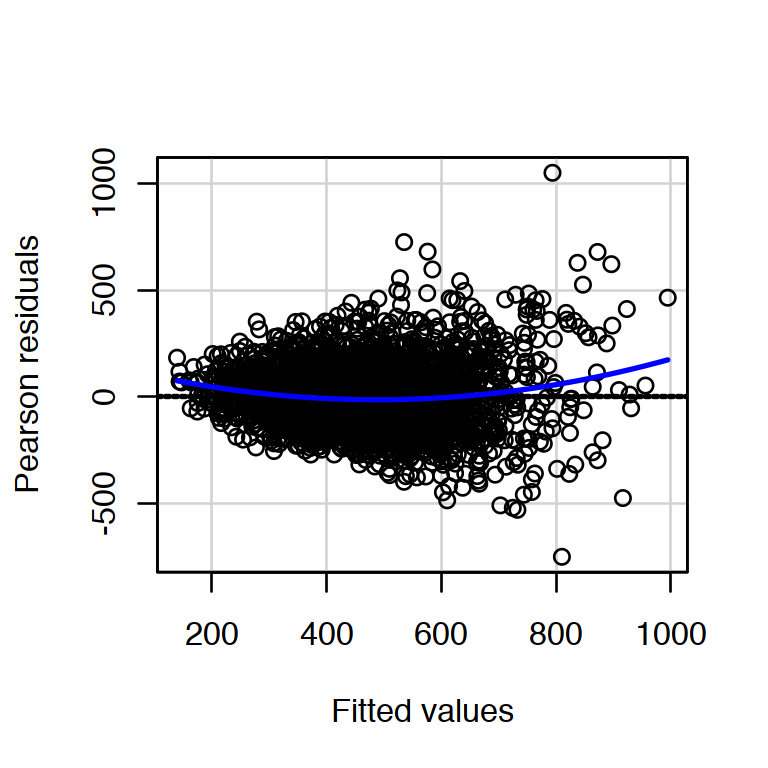
\includegraphics[width=0.9\linewidth]{hw_glm_2018_files/figure-latex/unnamed-chunk-6-1} \end{center}

\begin{Shaded}
\begin{Highlighting}[]
\KeywordTok{summary}\NormalTok{(fit}\FloatTok{.5}\NormalTok{)}
\end{Highlighting}
\end{Shaded}

\begin{verbatim}
## 
## Call:
## glm(formula = rvote ~ income.new, family = binomial(link = "logit"))
## 
## Deviance Residuals: 
##     Min       1Q   Median       3Q      Max  
## -1.4089  -1.1984   0.9623   1.1565   1.3650  
## 
## Coefficients:
##             Estimate Std. Error z value Pr(>|z|)    
## (Intercept)  0.04928    0.01724   2.859  0.00425 ** 
## income.new   0.24012    0.01559  15.398  < 2e-16 ***
## ---
## Signif. codes:  0 '***' 0.001 '**' 0.01 '*' 0.05 '.' 0.1 ' ' 1
## 
## (Dispersion parameter for binomial family taken to be 1)
## 
##     Null deviance: 19057  on 13756  degrees of freedom
## Residual deviance: 18815  on 13755  degrees of freedom
##   (21151 observations deleted due to missingness)
## AIC: 18819
## 
## Number of Fisher Scoring iterations: 4
\end{verbatim}

\begin{Shaded}
\begin{Highlighting}[]
\NormalTok{fit}\FloatTok{.6}\NormalTok{ =}\StringTok{ }\KeywordTok{glm}\NormalTok{(rvote }\OperatorTok{~}\StringTok{ }\NormalTok{income.new,}\DataTypeTok{family =} \KeywordTok{binomial}\NormalTok{(}\DataTypeTok{link =} \StringTok{"probit"}\NormalTok{))}
\KeywordTok{summary}\NormalTok{(fit}\FloatTok{.6}\NormalTok{)}
\end{Highlighting}
\end{Shaded}

\begin{verbatim}
## 
## Call:
## glm(formula = rvote ~ income.new, family = binomial(link = "probit"))
## 
## Deviance Residuals: 
##     Min       1Q   Median       3Q      Max  
## -1.4099  -1.1985   0.9615   1.1564   1.3652  
## 
## Coefficients:
##             Estimate Std. Error z value Pr(>|z|)    
## (Intercept) 0.031039   0.010761   2.884  0.00392 ** 
## income.new  0.150209   0.009691  15.500  < 2e-16 ***
## ---
## Signif. codes:  0 '***' 0.001 '**' 0.01 '*' 0.05 '.' 0.1 ' ' 1
## 
## (Dispersion parameter for binomial family taken to be 1)
## 
##     Null deviance: 19057  on 13756  degrees of freedom
## Residual deviance: 18815  on 13755  degrees of freedom
##   (21151 observations deleted due to missingness)
## AIC: 18819
## 
## Number of Fisher Scoring iterations: 3
\end{verbatim}

\begin{Shaded}
\begin{Highlighting}[]
\NormalTok{logitcoef =}\StringTok{ }\NormalTok{fit}\FloatTok{.5}\OperatorTok{$}\NormalTok{coefficients}
\NormalTok{probitcoef =}\StringTok{ }\NormalTok{fit}\FloatTok{.6}\OperatorTok{$}\NormalTok{coefficients}
\KeywordTok{print}\NormalTok{(}\StringTok{"the ratio of coefs in logit over coefs in probit is:"}\NormalTok{)}
\end{Highlighting}
\end{Shaded}

\begin{verbatim}
## [1] "the ratio of coefs in logit over coefs in probit is:"
\end{verbatim}

\begin{Shaded}
\begin{Highlighting}[]
\KeywordTok{print}\NormalTok{(}\KeywordTok{round}\NormalTok{(logitcoef}\OperatorTok{/}\NormalTok{probitcoef,}\DataTypeTok{digits =} \DecValTok{2}\NormalTok{))}
\end{Highlighting}
\end{Shaded}

\begin{verbatim}
## (Intercept)  income.new 
##        1.59        1.60
\end{verbatim}

\hypertarget{comparing-logit-and-probit-1}{%
\section{Comparing logit and
probit:}\label{comparing-logit-and-probit-1}}

construct a dataset where the logit and probit models give different
estimates.

\hypertarget{tobit-model-for-mixed-discrete-or-continuous-data}{%
\section{Tobit model for mixed discrete or continuous
data:}\label{tobit-model-for-mixed-discrete-or-continuous-data}}

experimental data from the National Supported Work example are available
in the folder \emph{lalonde}. Use the treatment indicator and
pre-treatment variables to predict post-treatment (1978) earnings using
a tobit model. Interpret the model coefficients.

\begin{itemize}
\tightlist
\item
  sample: 1 = NSW; 2 = CPS; 3 = PSID.
\item
  treat: 1 = experimental treatment group (NSW); 0 = comparison group
  (either from CPS or PSID) - Treatment took place in 1976 and 1977.
\item
  age = age in years
\item
  educ = years of schooling
\item
  black: 1 if black; 0 otherwise.
\item
  hisp: 1 if Hispanic; 0 otherwise.
\item
  married: 1 if married; 0 otherwise.
\item
  nodegree: 1 if no high school diploma; 0 otherwise.
\item
  re74, re75, re78: real earnings in 1974, 1975 and 1978
\item
  educ\_cat = 4 category education variable (1=\textless{}hs, 2=hs, 3=sm
  college, 4=college)
\end{itemize}

\begin{Shaded}
\begin{Highlighting}[]
\NormalTok{lalonde<-}\KeywordTok{read.dta}\NormalTok{(}\StringTok{"http://www.stat.columbia.edu/~gelman/arm/examples/lalonde/NSW.dw.obs.dta"}\NormalTok{)}
\CommentTok{## Check outcome distribution}
\KeywordTok{hist}\NormalTok{(lalonde}\OperatorTok{$}\NormalTok{re78)}
\end{Highlighting}
\end{Shaded}

\begin{center}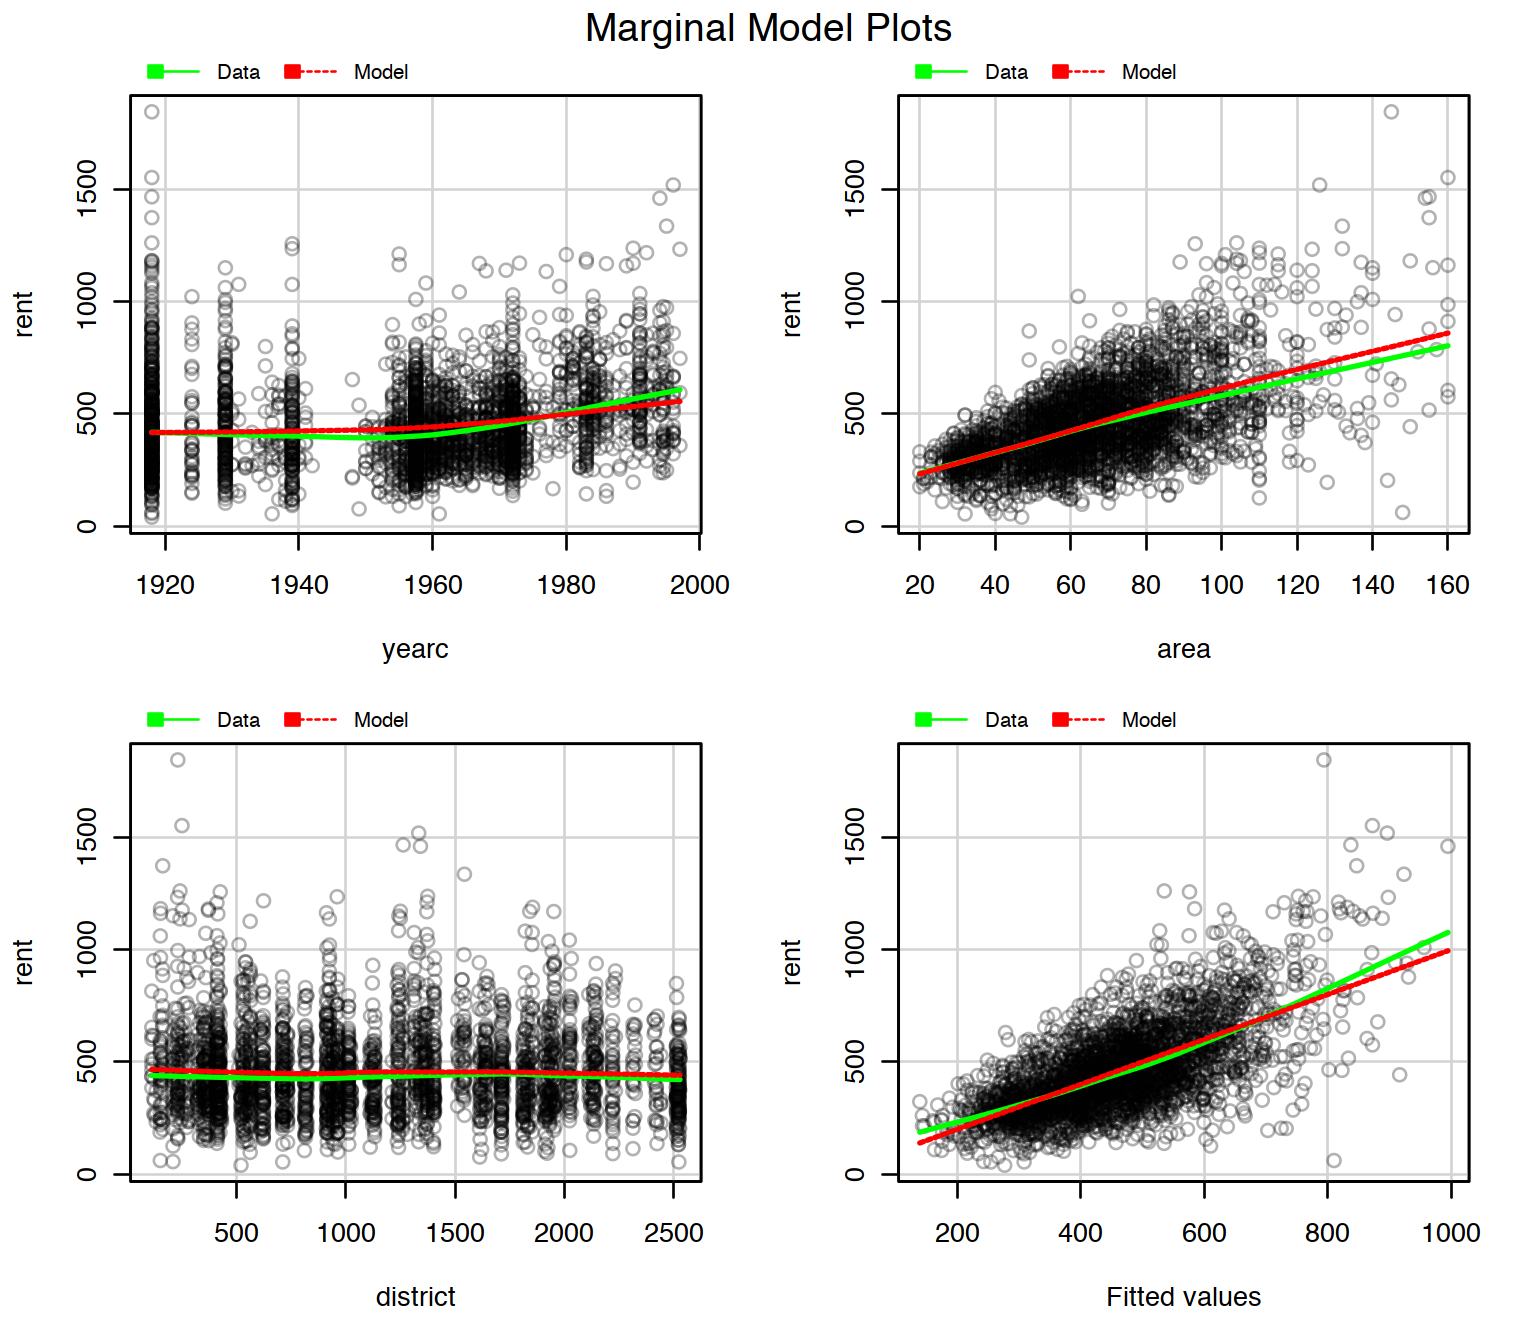
\includegraphics[width=0.9\linewidth]{hw_glm_2018_files/figure-latex/unnamed-chunk-7-1} \end{center}

\begin{Shaded}
\begin{Highlighting}[]
\CommentTok{## this in not a normal distribution}
\KeywordTok{summary}\NormalTok{(}\KeywordTok{censReg}\NormalTok{(}\DataTypeTok{data =}\NormalTok{ lalonde, re78 }\OperatorTok{~}\StringTok{ }\NormalTok{re74}\OperatorTok{+}\NormalTok{re75}\OperatorTok{+}\NormalTok{treat,}\DataTypeTok{left =} \DecValTok{0}\NormalTok{,}\DataTypeTok{right =} \OtherTok{Inf}\NormalTok{))}
\end{Highlighting}
\end{Shaded}

\begin{verbatim}
## 
## Call:
## censReg(formula = re78 ~ re74 + re75 + treat, left = 0, right = Inf, 
##     data = lalonde)
## 
## Observations:
##          Total  Left-censored     Uncensored Right-censored 
##          18667           2503          16164              0 
## 
## Coefficients:
##              Estimate Std. error t value Pr(> t)    
## (Intercept) 2.873e+03  1.180e+02   24.36  <2e-16 ***
## re74        2.689e-01  1.246e-02   21.58  <2e-16 ***
## re75        5.744e-01  1.274e-02   45.10  <2e-16 ***
## treat       6.977e+02  6.646e+02    1.05   0.294    
## logSigma    9.063e+00  5.731e-03 1581.30  <2e-16 ***
## ---
## Signif. codes:  0 '***' 0.001 '**' 0.01 '*' 0.05 '.' 0.1 ' ' 1
## 
## Newton-Raphson maximisation, 9 iterations
## Return code 1: gradient close to zero
## Log-likelihood: -172040.9 on 5 Df
\end{verbatim}

The model coef can be interpreted as a lm model of
\(\hat{y}^\star = X\hat{\beta}\) which means is a linear model with
respect to the latent variable \(y^{\star}\) but with a left cencored
condition when translating the result from \(y^{\star}\) to \(y\).

\hypertarget{robust-linear-regression-using-the-t-model}{%
\section{Robust linear regression using the t
model:}\label{robust-linear-regression-using-the-t-model}}

The csv file \emph{congress }has the votes for the Democratic and
Republican candidates in each U.S. congressional district in between
1896 and 1992, along with the parties' vote proportions and an indicator
for whether the incumbent was running for reelection. For your analysis,
just use the elections in 1986 and 1988 that were contested by both
parties in both years.

\begin{Shaded}
\begin{Highlighting}[]
\NormalTok{congress<-}\KeywordTok{read.csv}\NormalTok{(}\StringTok{"congress.csv"}\NormalTok{,}\DataTypeTok{header=}\OtherTok{TRUE}\NormalTok{)}
\NormalTok{congress =}\StringTok{ }\NormalTok{congress }\OperatorTok\StringTok{ }\NormalTok{dplyr}\OperatorTok{::}\KeywordTok{filter}\NormalTok{(year }\OperatorTok\StringTok{ }\KeywordTok{c}\NormalTok{(}\DecValTok{1986}\NormalTok{,}\DecValTok{1988}\NormalTok{),contested }\OperatorTok{==}\StringTok{ }\OtherTok{TRUE}\NormalTok{)}\OperatorTok\KeywordTok{select}\NormalTok{(x1,x2,incumbent,year,Dem_pct)}

\NormalTok{congress =}\StringTok{ }\KeywordTok{full_join}\NormalTok{(congress}\OperatorTok\KeywordTok{filter}\NormalTok{(year }\OperatorTok{==}\StringTok{ }\DecValTok{1986}\NormalTok{)}\OperatorTok\KeywordTok{pivot_wider}\NormalTok{(}\DataTypeTok{names_from =}\NormalTok{ year,}\DataTypeTok{values_from =}\NormalTok{ Dem_pct)}\OperatorTok\KeywordTok{rename}\NormalTok{(}\StringTok{`}\DataTypeTok{1986incumbent}\StringTok{`}\NormalTok{ =}\StringTok{ }\NormalTok{incumbent),congress}\OperatorTok\KeywordTok{filter}\NormalTok{(year }\OperatorTok{==}\StringTok{ }\DecValTok{1988}\NormalTok{)}\OperatorTok\KeywordTok{pivot_wider}\NormalTok{(}\DataTypeTok{names_from =}\NormalTok{ year,}\DataTypeTok{values_from =}\NormalTok{ Dem_pct)}\OperatorTok\KeywordTok{rename}\NormalTok{(}\StringTok{`}\DataTypeTok{1988incumbent}\StringTok{`}\NormalTok{ =}\StringTok{ }\NormalTok{incumbent))}
\end{Highlighting}
\end{Shaded}

\begin{verbatim}
## Joining, by = c("x1", "x2")
\end{verbatim}

\begin{Shaded}
\begin{Highlighting}[]
\CommentTok{#unique(congress$year)}
\end{Highlighting}
\end{Shaded}

\begin{enumerate}
\def\labelenumi{\arabic{enumi}.}
\tightlist
\item
  Fit a linear regression (with the usual normal-distribution model for
  the errors) predicting 1988 Democratic vote share from the other
  variables and assess model fit.
\end{enumerate}

\begin{Shaded}
\begin{Highlighting}[]
\KeywordTok{summary}\NormalTok{(fit}\FloatTok{.7}\NormalTok{ <-}\StringTok{ }\KeywordTok{lm}\NormalTok{(}\DataTypeTok{data =}\NormalTok{ congress,}\StringTok{`}\DataTypeTok{1988}\StringTok{`}\OperatorTok{~}\NormalTok{.))}
\end{Highlighting}
\end{Shaded}

\begin{verbatim}
## 
## Call:
## lm(formula = `1988` ~ ., data = congress)
## 
## Residuals:
##      Min       1Q   Median       3Q      Max 
## -0.16614 -0.03293 -0.00043  0.03594  0.19754 
## 
## Coefficients:
##                   Estimate Std. Error t value Pr(>|t|)    
## (Intercept)      0.1426014  0.0219306   6.502 3.27e-10 ***
## x1               0.0003460  0.0001667   2.076   0.0388 *  
## x2              -0.0000199  0.0002516  -0.079   0.9370    
## `1986incumbent` -0.0401303  0.0081039  -4.952 1.22e-06 ***
## `1986`           0.6746752  0.0405806  16.626  < 2e-16 ***
## `1988incumbent`  0.0962035  0.0075444  12.752  < 2e-16 ***
## ---
## Signif. codes:  0 '***' 0.001 '**' 0.01 '*' 0.05 '.' 0.1 ' ' 1
## 
## Residual standard error: 0.06319 on 302 degrees of freedom
##   (87 observations deleted due to missingness)
## Multiple R-squared:  0.889,  Adjusted R-squared:  0.8871 
## F-statistic: 483.7 on 5 and 302 DF,  p-value: < 2.2e-16
\end{verbatim}

\begin{Shaded}
\begin{Highlighting}[]
\KeywordTok{ggplot}\NormalTok{(fit}\FloatTok{.7}\NormalTok{)}\OperatorTok{+}\KeywordTok{aes}\NormalTok{(}\DataTypeTok{x=}\NormalTok{.fitted,}\DataTypeTok{y=}\NormalTok{.resid)}\OperatorTok{+}\KeywordTok{geom_point}\NormalTok{()}\OperatorTok{+}\KeywordTok{geom_smooth}\NormalTok{(}\DataTypeTok{method =} \StringTok{"loess"}\NormalTok{)}
\end{Highlighting}
\end{Shaded}

\begin{center}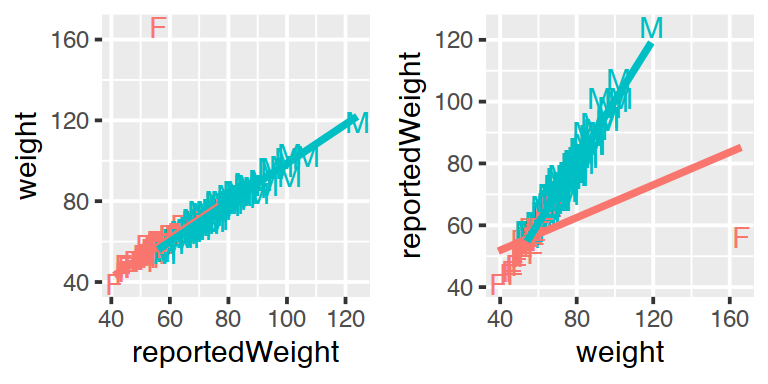
\includegraphics[width=0.9\linewidth]{hw_glm_2018_files/figure-latex/unnamed-chunk-9-1} \end{center}

\begin{enumerate}
\def\labelenumi{\arabic{enumi}.}
\setcounter{enumi}{1}
\tightlist
\item
  Fit a t-regression model predicting 1988 Democratic vote share from
  the other variables and assess model fit; to fit this model in R you
  can use the \emph{\texttt{vglm()}} function in the VGLM package or
  \emph{\texttt{tlm()}} function in the hett package.
\end{enumerate}

\begin{Shaded}
\begin{Highlighting}[]
\KeywordTok{summary}\NormalTok{(fit}\FloatTok{.8}\NormalTok{ <-}\StringTok{ }\KeywordTok{vglm}\NormalTok{(}\DataTypeTok{data =}\NormalTok{ congress,}\StringTok{`}\DataTypeTok{1988}\StringTok{`}\OperatorTok{~}\NormalTok{.,}\DataTypeTok{family =}\NormalTok{gaussianff ))}
\end{Highlighting}
\end{Shaded}

\begin{verbatim}
## 
## Call:
## vglm(formula = `1988` ~ ., family = gaussianff, data = congress)
## 
## Pearson residuals:
##                 Min      1Q    Median     3Q   Max
## mean        -2.6553 -0.5263 -0.006873 0.5744 3.157
## loglink(sd) -0.7071 -0.6627 -0.502176 0.1796 6.341
## 
## Coefficients: 
##                   Estimate Std. Error z value Pr(>|z|)    
## (Intercept):1    0.1426014  0.0217164   6.567 5.15e-11 ***
## (Intercept):2   -2.7715142  0.0402911 -68.787  < 2e-16 ***
## x1               0.0003460  0.0001650   2.096   0.0361 *  
## x2              -0.0000199  0.0002491  -0.080   0.9363    
## `1986incumbent` -0.0401303  0.0080248  -5.001 5.71e-07 ***
## `1986`           0.6746752  0.0401843  16.790  < 2e-16 ***
## `1988incumbent`  0.0962035  0.0074707  12.877  < 2e-16 ***
## ---
## Signif. codes:  0 '***' 0.001 '**' 0.01 '*' 0.05 '.' 0.1 ' ' 1
## 
## Names of linear predictors: mean, loglink(sd)
## 
## Log-likelihood: 416.5933 on 609 degrees of freedom
## 
## Number of Fisher scoring iterations: 7 
## 
## No Hauck-Donner effect found in any of the estimates
\end{verbatim}

\begin{Shaded}
\begin{Highlighting}[]
\CommentTok{#anova(fit.8,fit.7)}
\KeywordTok{ggplot}\NormalTok{()}\OperatorTok{+}\KeywordTok{aes}\NormalTok{(}\DataTypeTok{x=}\KeywordTok{fitted}\NormalTok{(fit}\FloatTok{.8}\NormalTok{),}\DataTypeTok{y=}\KeywordTok{residuals}\NormalTok{(fit}\FloatTok{.8}\NormalTok{)[,}\DecValTok{1}\NormalTok{])}\OperatorTok{+}\KeywordTok{geom_point}\NormalTok{()}\OperatorTok{+}\KeywordTok{geom_smooth}\NormalTok{(}\DataTypeTok{method =} \StringTok{"loess"}\NormalTok{)}
\end{Highlighting}
\end{Shaded}

\begin{center}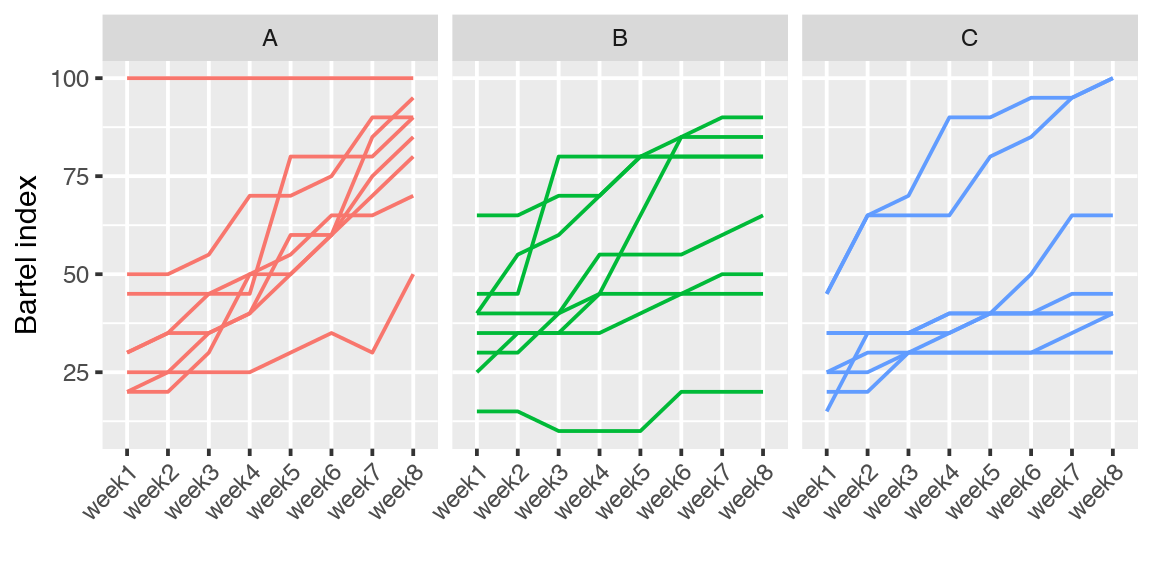
\includegraphics[width=0.9\linewidth]{hw_glm_2018_files/figure-latex/unnamed-chunk-10-1} \end{center}

\begin{Shaded}
\begin{Highlighting}[]
\KeywordTok{rSquared}\NormalTok{(}\DataTypeTok{resid =} \KeywordTok{residuals}\NormalTok{(fit}\FloatTok{.8}\NormalTok{)[,}\DecValTok{1}\NormalTok{],}\DataTypeTok{y =} \KeywordTok{drop_na}\NormalTok{(}\KeywordTok{select}\NormalTok{(congress,}\StringTok{`}\DataTypeTok{1988}\StringTok{`}\NormalTok{))}\OperatorTok\KeywordTok{pull}\NormalTok{())}
\end{Highlighting}
\end{Shaded}

\begin{verbatim}
##           [,1]
## [1,] 0.9048855
\end{verbatim}

\begin{enumerate}
\def\labelenumi{\arabic{enumi}.}
\setcounter{enumi}{2}
\tightlist
\item
  Which model do you prefer?
\end{enumerate}

\hypertarget{robust-regression-for-binary-data-using-the-robit-model}{%
\section{Robust regression for binary data using the robit
model:}\label{robust-regression-for-binary-data-using-the-robit-model}}

Use the same data as the previous example with the goal instead of
predicting for each district whether it was won by the Democratic or
Republican candidate.

\begin{enumerate}
\def\labelenumi{\arabic{enumi}.}
\tightlist
\item
  Fit a standard logistic or probit regression and assess model fit.
\end{enumerate}

\begin{Shaded}
\begin{Highlighting}[]
\NormalTok{congressbi =}\StringTok{ }\NormalTok{congress}\OperatorTok\KeywordTok{mutate}\NormalTok{(}\StringTok{`}\DataTypeTok{1988}\StringTok{`}\NormalTok{ =}\StringTok{ }\KeywordTok{if_else}\NormalTok{(}\StringTok{`}\DataTypeTok{1988}\StringTok{`}\OperatorTok{>}\FloatTok{0.5}\NormalTok{,}\FloatTok{1.0}\NormalTok{,}\FloatTok{0.0}\NormalTok{))}
\KeywordTok{summary}\NormalTok{(fit}\FloatTok{.9}\NormalTok{ <-}\StringTok{  }\KeywordTok{glm}\NormalTok{(}\DataTypeTok{data =}\NormalTok{ congressbi , }\StringTok{`}\DataTypeTok{1988}\StringTok{`}\OperatorTok{~}\StringTok{ }\NormalTok{. ,}\DataTypeTok{family =} \KeywordTok{binomial}\NormalTok{(}\DataTypeTok{link =} \StringTok{"logit"}\NormalTok{)))}
\end{Highlighting}
\end{Shaded}

\begin{verbatim}
## 
## Call:
## glm(formula = `1988` ~ ., family = binomial(link = "logit"), 
##     data = congressbi)
## 
## Deviance Residuals: 
##      Min        1Q    Median        3Q       Max  
## -2.56350  -0.11141   0.02767   0.10582   2.56281  
## 
## Coefficients:
##                   Estimate Std. Error z value Pr(>|z|)    
## (Intercept)     -10.172569   2.796629  -3.637 0.000275 ***
## x1                0.003266   0.018266   0.179 0.858093    
## x2               -0.016727   0.023756  -0.704 0.481368    
## `1986incumbent`  -1.449757   0.855001  -1.696 0.089958 .  
## `1986`           20.534859   5.112120   4.017  5.9e-05 ***
## `1988incumbent`   3.023907   0.788417   3.835 0.000125 ***
## ---
## Signif. codes:  0 '***' 0.001 '**' 0.01 '*' 0.05 '.' 0.1 ' ' 1
## 
## (Dispersion parameter for binomial family taken to be 1)
## 
##     Null deviance: 425.406  on 307  degrees of freedom
## Residual deviance:  56.159  on 302  degrees of freedom
##   (87 observations deleted due to missingness)
## AIC: 68.159
## 
## Number of Fisher Scoring iterations: 8
\end{verbatim}

\begin{Shaded}
\begin{Highlighting}[]
\KeywordTok{binnedplot}\NormalTok{(}\DataTypeTok{x =}\NormalTok{ fit}\FloatTok{.9}\OperatorTok{$}\NormalTok{fitted,}\DataTypeTok{y =}\NormalTok{ fit}\FloatTok{.9}\OperatorTok{$}\NormalTok{resid)}
\end{Highlighting}
\end{Shaded}

\begin{center}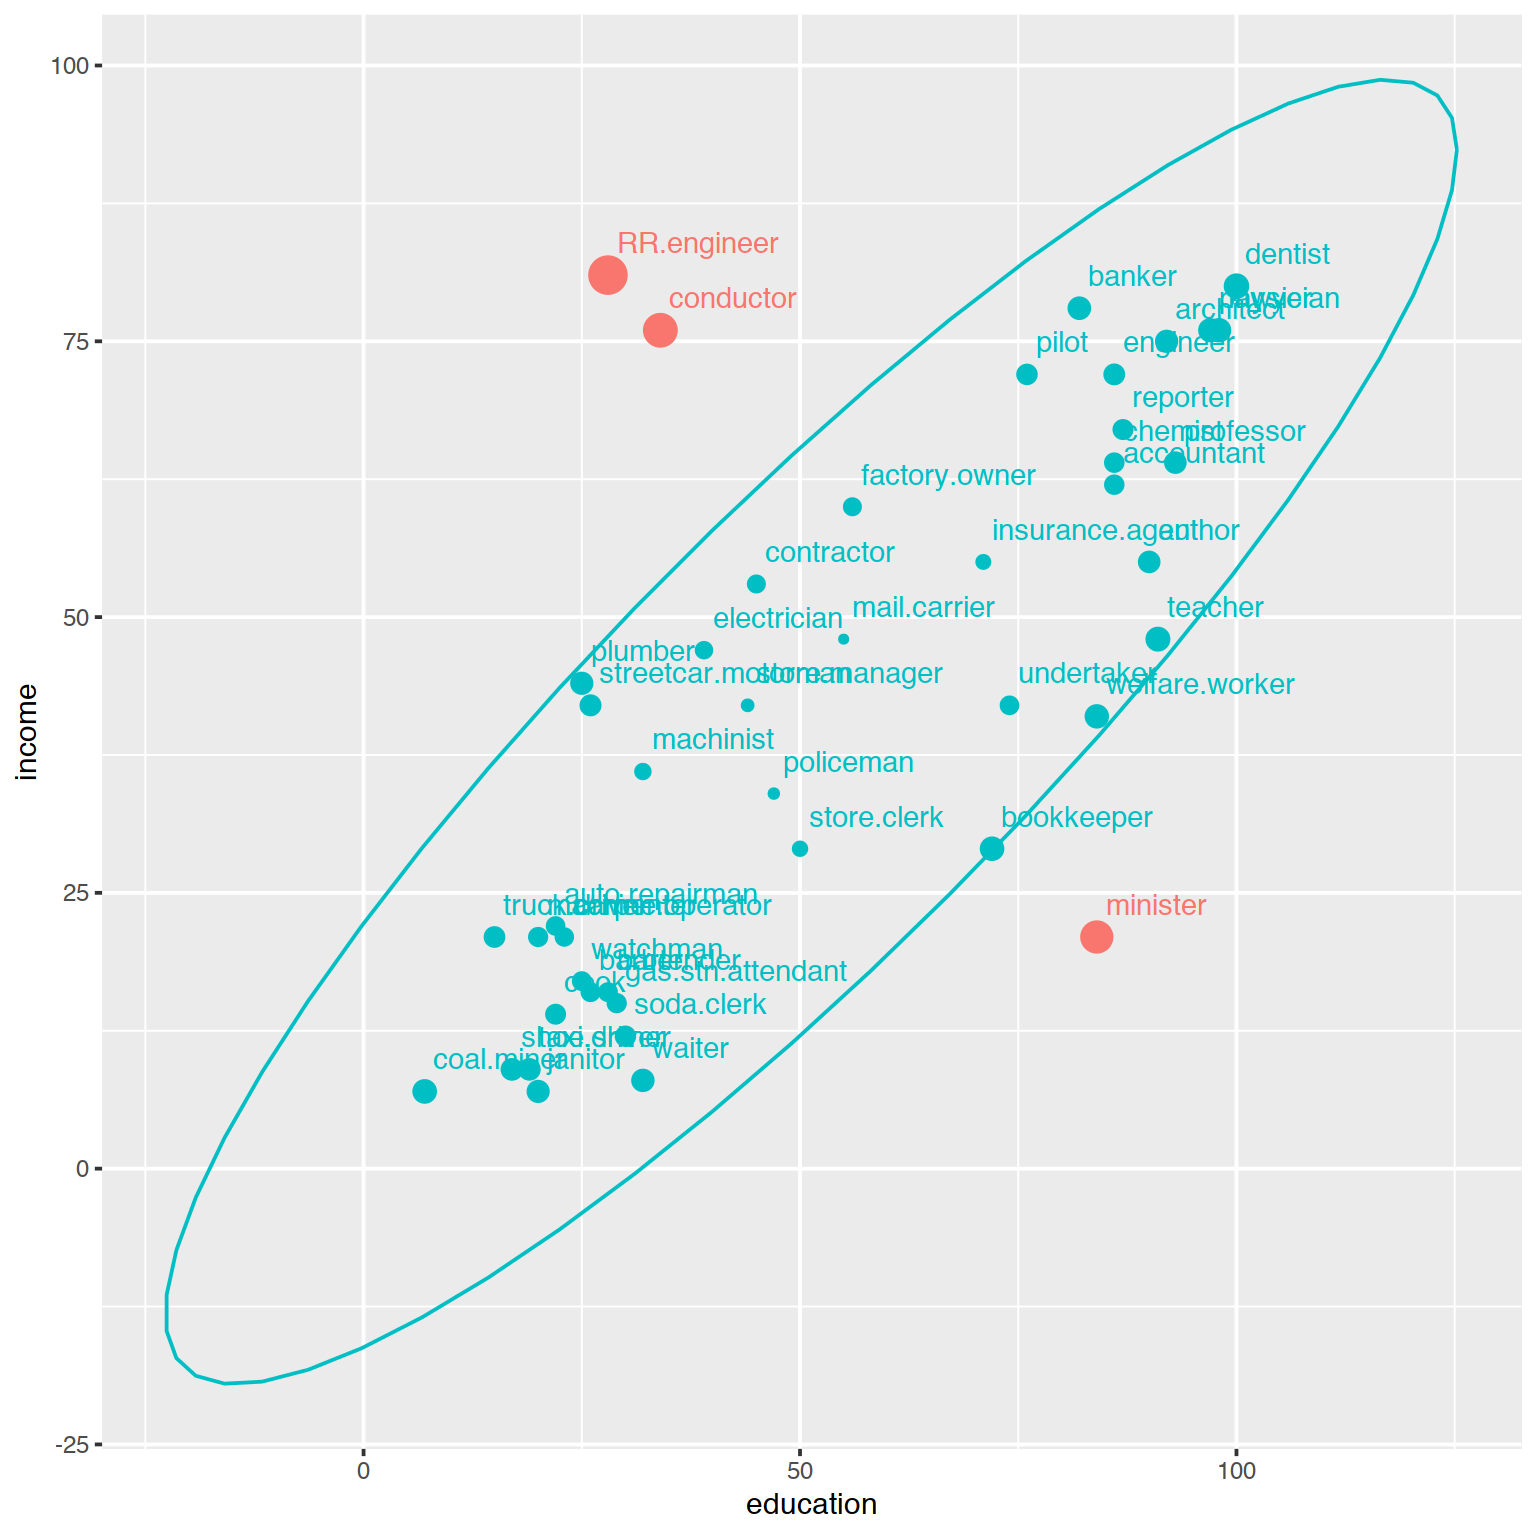
\includegraphics[width=0.9\linewidth]{hw_glm_2018_files/figure-latex/unnamed-chunk-11-1} \end{center}

\begin{enumerate}
\def\labelenumi{\arabic{enumi}.}
\setcounter{enumi}{1}
\item
  Fit a robit regression and assess model fit.
\item
  Which model do you prefer?
\end{enumerate}

\hypertarget{salmonellla}{%
\section{Salmonellla}\label{salmonellla}}

The \emph{\texttt{salmonella}} data was collected in a salmonella
reverse mutagenicity assay. The predictor is the dose level of quinoline
and the response is the numbers of revertant colonies of TA98 salmonella
observed on each of three replicate plates. Show that a Poisson GLM is
inadequate and that some overdispersion must be allowed for. Do not
forget to check out other reasons for a high deviance.

\begin{Shaded}
\begin{Highlighting}[]
\NormalTok{salmonella =}\StringTok{ }\KeywordTok{force}\NormalTok{(salmonella)}
\CommentTok{#?salmonella}
\end{Highlighting}
\end{Shaded}

When you plot the data you see that the number of colonies as a function
of dose is not monotonic especially around the dose of 1000.

\begin{Shaded}
\begin{Highlighting}[]
\KeywordTok{ggplot}\NormalTok{(salmonella)}\OperatorTok{+}\KeywordTok{aes}\NormalTok{(}\DataTypeTok{x =}\NormalTok{ dose,}\DataTypeTok{y =}\NormalTok{ colonies)}\OperatorTok{+}\KeywordTok{geom_point}\NormalTok{()}
\end{Highlighting}
\end{Shaded}

\begin{center}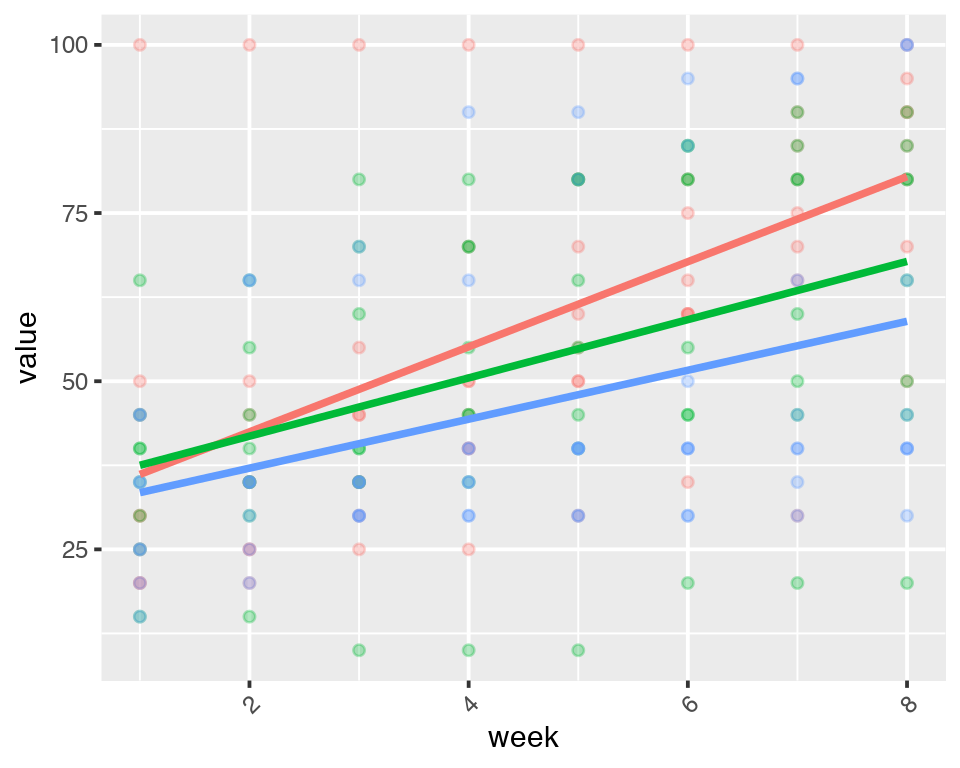
\includegraphics[width=0.9\linewidth]{hw_glm_2018_files/figure-latex/unnamed-chunk-15-1} \end{center}

Since we are fitting log linear model we should look at the data on log
scale. Also becase the dose is not equally spaced on the raw scale it
may be better to plot it on the log scale as well.

\begin{Shaded}
\begin{Highlighting}[]
\KeywordTok{ggplot}\NormalTok{(salmonella)}\OperatorTok{+}\KeywordTok{aes}\NormalTok{(}\DataTypeTok{x =} \KeywordTok{log}\NormalTok{(dose),}\DataTypeTok{y =} \KeywordTok{log}\NormalTok{(colonies))}\OperatorTok{+}\KeywordTok{geom_point}\NormalTok{()}
\end{Highlighting}
\end{Shaded}

\begin{center}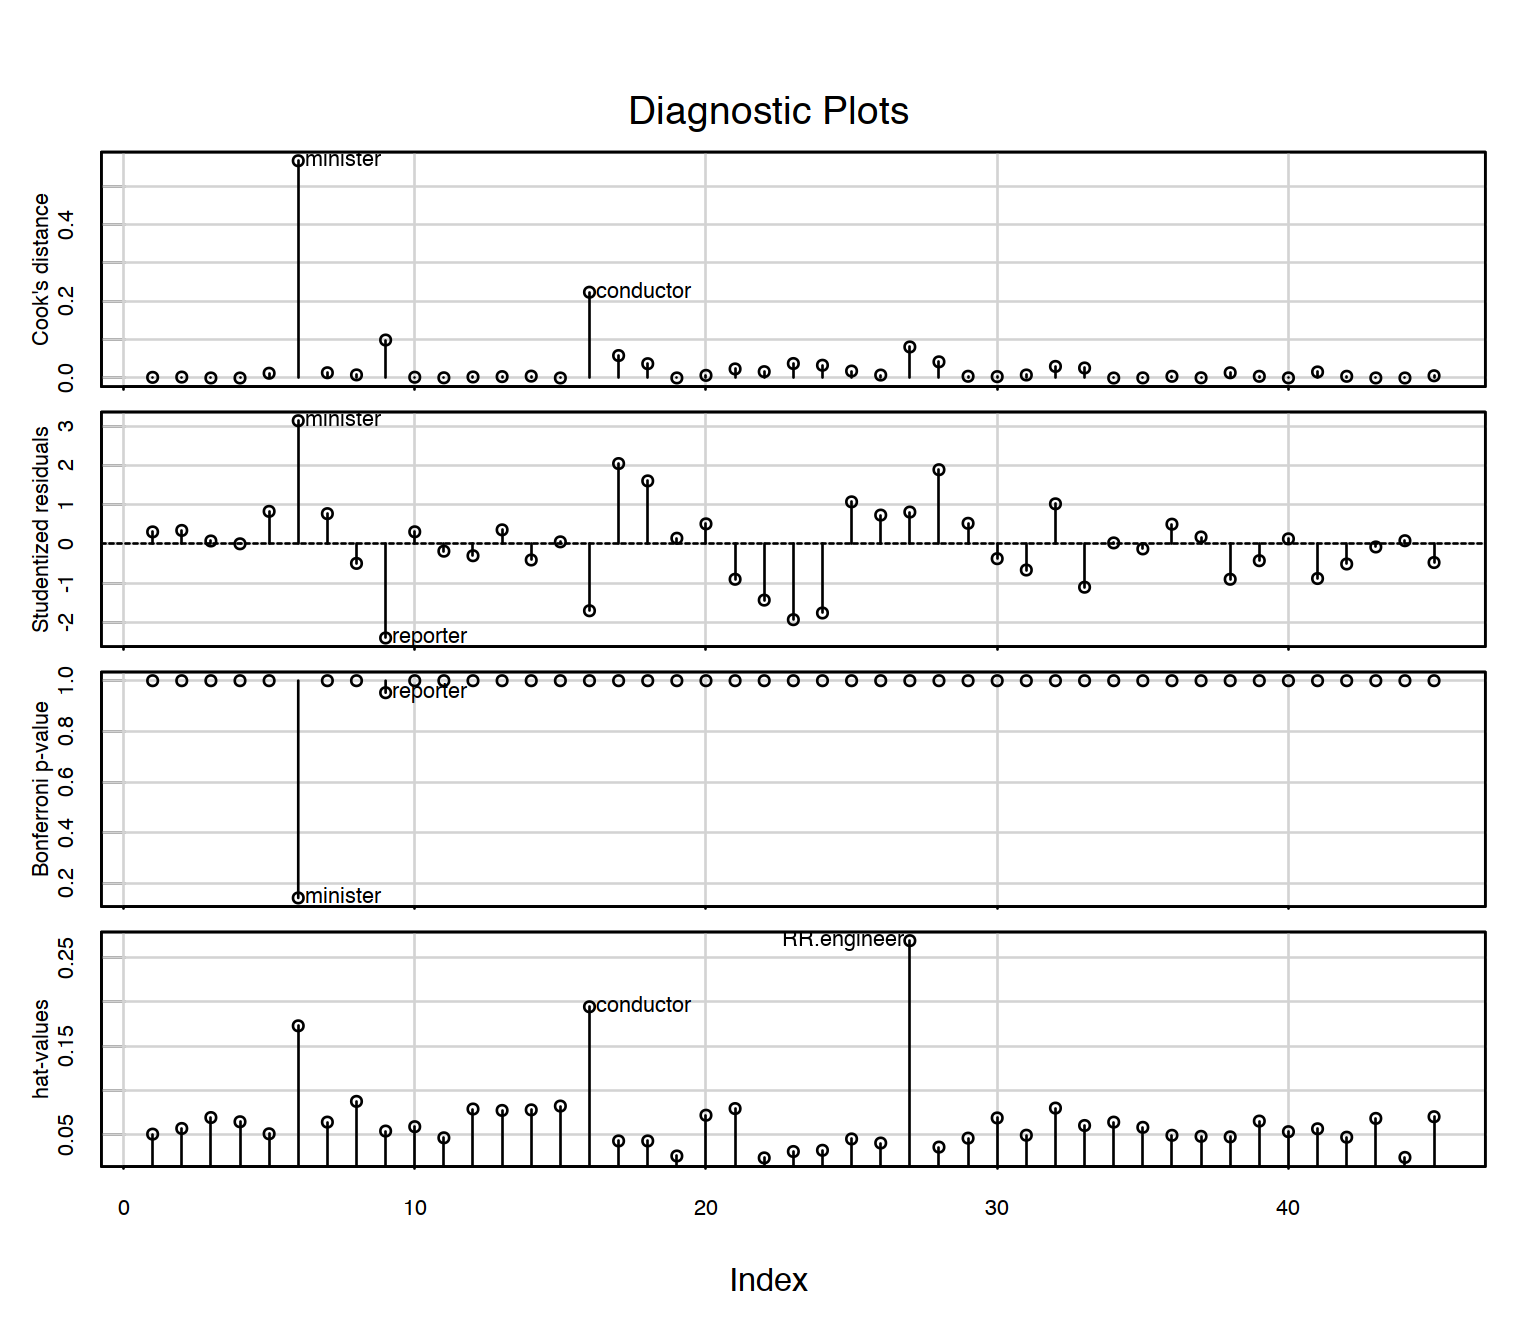
\includegraphics[width=0.9\linewidth]{hw_glm_2018_files/figure-latex/unnamed-chunk-16-1} \end{center}

This shows that the trend is not monotonic. Hence when you fit the model
and look at the residual you will see a trend.

\begin{Shaded}
\begin{Highlighting}[]
\NormalTok{fit}\FloatTok{.10}\NormalTok{ <-}\StringTok{ }\KeywordTok{glm}\NormalTok{(}\DataTypeTok{data =}\NormalTok{ salmonella,colonies }\OperatorTok{~}\StringTok{ }\NormalTok{dose,}\DataTypeTok{family =} \KeywordTok{poisson}\NormalTok{(}\DataTypeTok{link =} \StringTok{"log"}\NormalTok{))}
\KeywordTok{summary}\NormalTok{(fit}\FloatTok{.10}\NormalTok{)}
\end{Highlighting}
\end{Shaded}

\begin{verbatim}
## 
## Call:
## glm(formula = colonies ~ dose, family = poisson(link = "log"), 
##     data = salmonella)
## 
## Deviance Residuals: 
##     Min       1Q   Median       3Q      Max  
## -2.6482  -1.8225  -0.2993   1.2917   5.1861  
## 
## Coefficients:
##              Estimate Std. Error z value Pr(>|z|)    
## (Intercept) 3.3219950  0.0540292  61.485   <2e-16 ***
## dose        0.0001901  0.0001172   1.622    0.105    
## ---
## Signif. codes:  0 '***' 0.001 '**' 0.01 '*' 0.05 '.' 0.1 ' ' 1
## 
## (Dispersion parameter for poisson family taken to be 1)
## 
##     Null deviance: 78.358  on 17  degrees of freedom
## Residual deviance: 75.806  on 16  degrees of freedom
## AIC: 172.34
## 
## Number of Fisher Scoring iterations: 4
\end{verbatim}

\begin{Shaded}
\begin{Highlighting}[]
\KeywordTok{ggplot}\NormalTok{(fit}\FloatTok{.10}\NormalTok{)}\OperatorTok{+}\KeywordTok{aes}\NormalTok{(}\DataTypeTok{x =}\NormalTok{ .fitted,}\DataTypeTok{y =}\NormalTok{.stdresid)}\OperatorTok{+}\KeywordTok{geom_point}\NormalTok{()}
\end{Highlighting}
\end{Shaded}

\begin{center}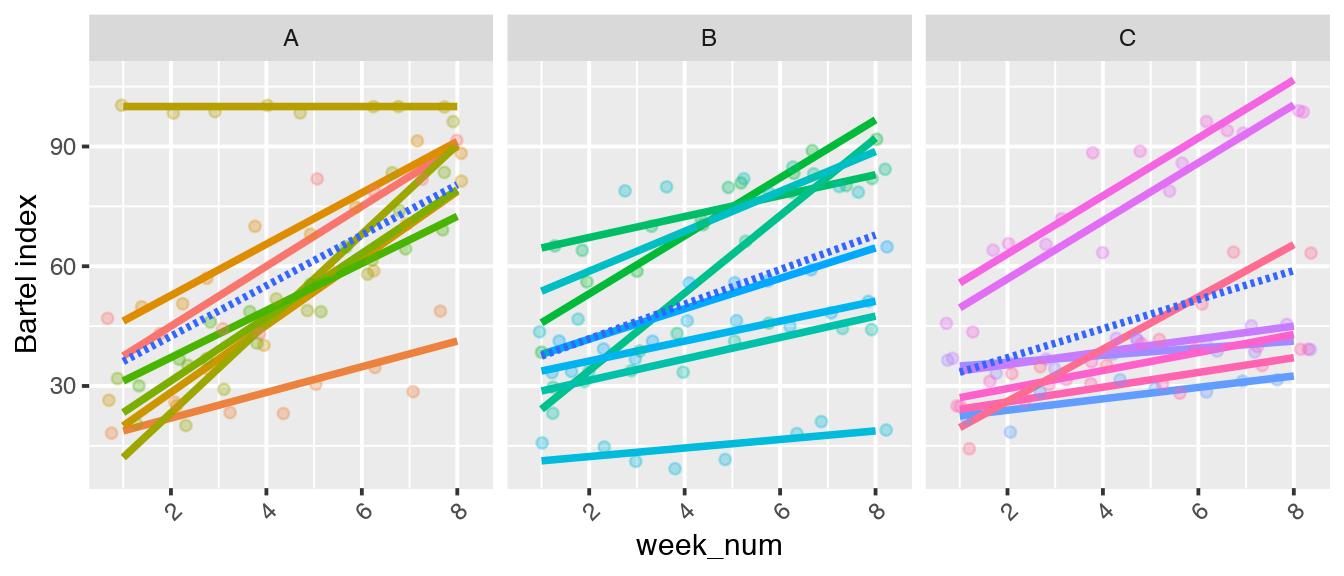
\includegraphics[width=0.9\linewidth]{hw_glm_2018_files/figure-latex/unnamed-chunk-17-1} \end{center}

The lack of fit is also evident if we plot the fitted line onto the
data.

How do we adress this problem? The serious problem to address is the
nonlinear trend of dose ranther than the overdispersion since the line
is missing the points. Let's add a beny line with 4th order polynomial.

The resulting residual looks nice and if you plot it on the raw data.
Whether the trend makes real contextual sense will need to be validated
but for the given data it looks feasible.

Dispite the fit, the overdispersion still exists so we'd be better off
using the quasi Poisson model.

\hypertarget{ships}{%
\section{Ships}\label{ships}}

The \texttt{ships} dataset found in the MASS package gives the number of
damage incidents and aggregate months of service for different types of
ships broken down by year of construction and period of operation.

\begin{Shaded}
\begin{Highlighting}[]
\CommentTok{#data(ships)}
\CommentTok{#?ships}
\end{Highlighting}
\end{Shaded}

Develop a model for the rate of incidents, describing the effect of the
important predictors.

\hypertarget{australian-health-survey}{%
\section{Australian Health Survey}\label{australian-health-survey}}

The \texttt{dvisits} data comes from the Australian Health Survey of
1977-78 and consist of 5190 single adults where young and old have been
oversampled.

\begin{Shaded}
\begin{Highlighting}[]
\CommentTok{#data(dvisits)}
\end{Highlighting}
\end{Shaded}

\begin{enumerate}
\def\labelenumi{\arabic{enumi}.}
\item
  Build a Poisson regression model with \emph{\texttt{doctorco}} as the
  response and \emph{\texttt{sex}, \texttt{age}, \texttt{agesq},
  \texttt{income}, \texttt{levyplus}, \texttt{freepoor},
  \texttt{freerepa}, \texttt{illness}, \texttt{actdays},
  \texttt{hscore}, \texttt{chcond1} and \texttt{chcond2}} as possible
  predictor variables. Considering the deviance of this model, does this
  model fit the data?
\item
  Plot the residuals and the fitted values-why are there lines of
  observations on the plot?
\item
  What sort of person would be predicted to visit the doctor the most
  under your selected model?
\item
  For the last person in the dataset, compute the predicted probability
  distribution for their visits to the doctor, i.e., give the
  probability they visit 0,1,2, etc. times.
\item
  Fit a comparable (Gaussian) linear model and graphically compare the
  fits. Describe how they differ.
\end{enumerate}


\end{document}
